\documentclass{beamer}
\usepackage[utf8]{inputenc}
\usepackage{hyperref}
%\usepackage{minted}\\
\usepackage{csvsimple}

\graphicspath{{img/}}

\title[Summary]{Systematic Mapping Study on Megamodels}
\author{Matthias Barde \& Marco Brack, University of Koblenz-Landau}
\institute{SLE course SS 2016 (\url{http://www.softlang.org/course:sle16})}
\date{2016-06-16}

\addtobeamertemplate{navigation symbols}{}{%
    \usebeamerfont{footline}%
    \usebeamercolor[fg]{footline}%
    \hspace{1em}%
    \insertframenumber/\inserttotalframenumber
}

\begin{document}

\begin{frame}
\titlepage
\end{frame}


\begin{frame}{Systematic Mapping Study}
\begin{figure}
	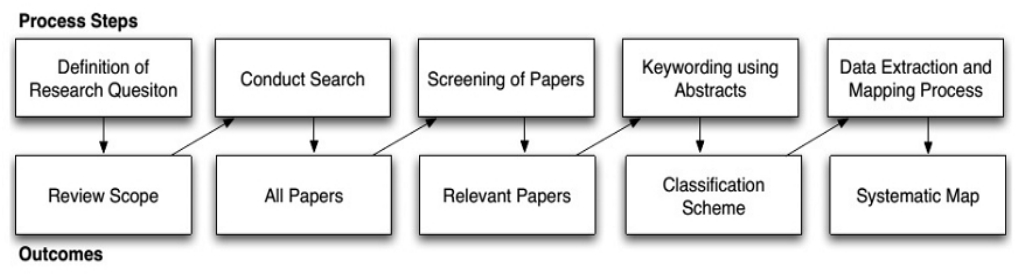
\includegraphics[width=1.0\textwidth]{sms_full}
\end{figure}
\end{frame}

\begin{frame}{Systematic Mapping Study}
\begin{figure}
	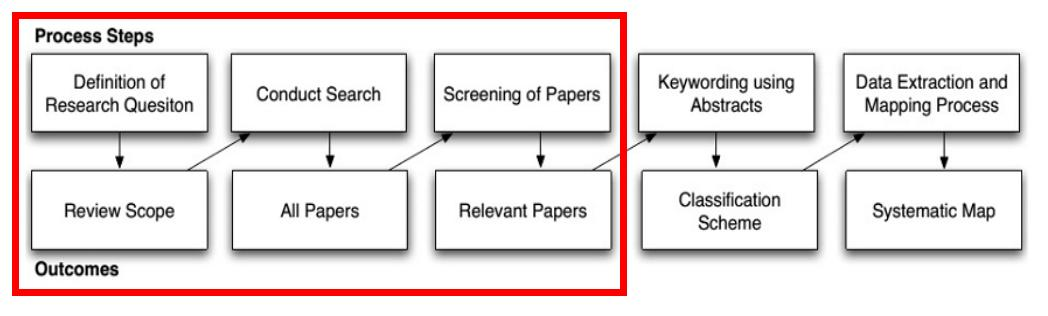
\includegraphics[width=1.0\textwidth]{sms_part_marked}
\end{figure}
\end{frame}

\begin{frame}{Research Questions}
\begin{enumerate}
	\item How do researchers define megamodeling?
	\item What kinds of model elements are used?
	\item How did the field of megamodeling evolve?
	\item Do the megamodels have any practical purpose?
	\item Do the megamodels reuse existing technology?	
\end{enumerate}
\end{frame}

\begin{frame}{Review Scope \& Conduct Search}

\begin{block}{Scope}
\begin{itemize}
	\item Papers cited in \textit{An Abstract View on Megamodeling Approaches} by Ralf Lämmel and Vadim Zaytsev \footnote{\url{http://softlang.uni-koblenz.de/megamodeling-in-the-wild/}}
	\item Elsevier
	\item Springer
	\item IEEE
	\item ACM
	\item DLBP
	\item Google Scholar as search engine
\end{itemize}
\end{block}

\begin{block}{Search query}
Term \textit{megamodel} must be contained in title or abstract.
\end{block}

\end{frame}

% Show collected papers as list at least one time.
\begin{frame}{All papers I}
22 papers, from 1974 to 2015
\begin{figure}
	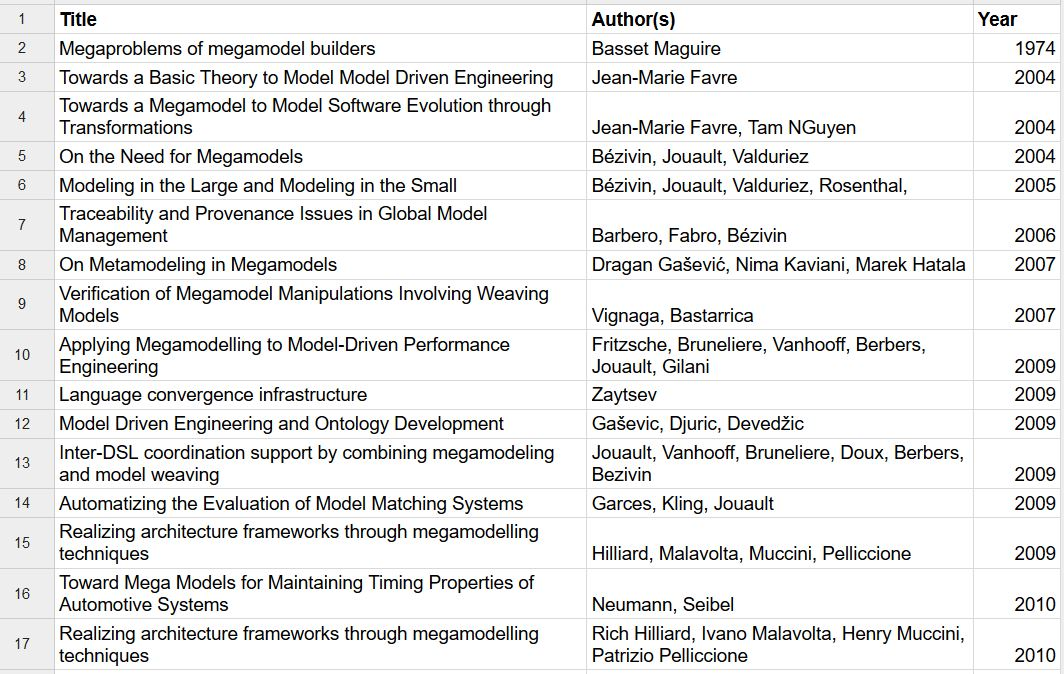
\includegraphics[width=1.0\textwidth]{all_papers_1}
\end{figure}
\end{frame}

\begin{frame}{All papers II}
\begin{figure}
	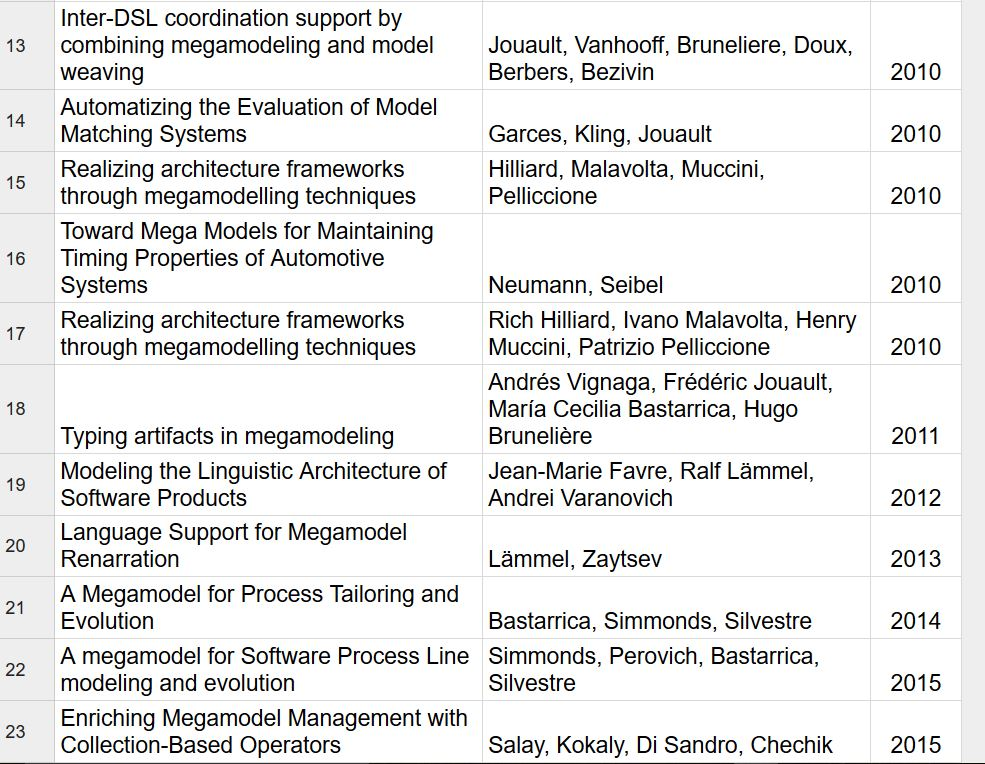
\includegraphics[width=1.0\textwidth]{all_papers_2}
\end{figure}
\end{frame}

\begin{frame}{Screening}
\begin{block}{Checking content of all papers:}
\begin{itemize}
	\item Abstract
	\item Introduction
	\item Conclusion
\end{itemize}
\end{block}
\vspace{1cm}
\large{$\rightarrow$ Can they contribute to our Research} Questions?\\
\large{$\rightarrow$ Short relevance analysis of each paper}
\end{frame}

\begin{frame}{Relevant papers}
\begin{itemize}
	\item Removed papers which do not contribute to any Research Question $\rightarrow$ \textit{Exclusion criterium}
	\item Number of papers reduced to 20
	\begin{itemize}
		\item 6 contribute to every Research Question
		\item 19 contribute to more than 2 (of 5) Research Questions
	\end{itemize}
\end{itemize}

\end{frame}

\begin{frame}{Future steps}
\begin{figure}
	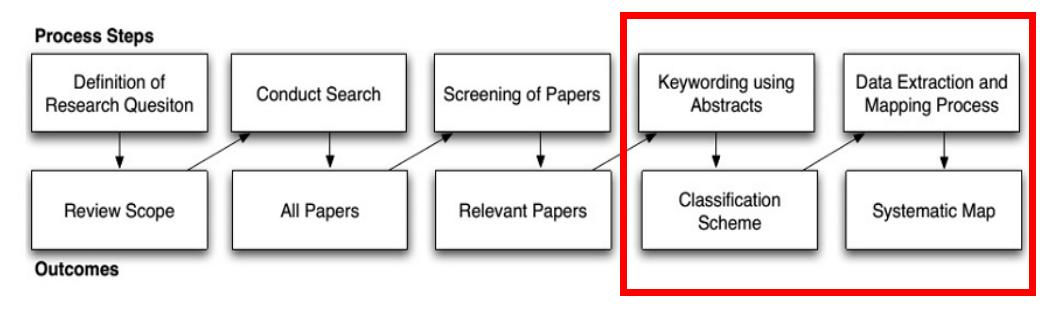
\includegraphics[width=1.0\textwidth]{sms_part_marked_2}
\end{figure}
\end{frame}

\begin{frame}
\begin{center}
	\huge{Final frame}
\end{center}
\end{frame}

\end{document}
